%%%%%%%%%%%%%%%%%%%%%%%%%%%%%%%%%%%%%%%%%%%%%%%
%%% Template for lab reports used at STIMA
%%%%%%%%%%%%%%%%%%%%%%%%%%%%%%%%%%%%%%%%%%%%%%%

%%%%%%%%%%%%%%%%%%%%%%%%%%%%%% Sets the document class for the document
% Openany is added to remove the book style of starting every new chapter on an odd page (not needed for reports)
\documentclass[10pt,english, openany]{book}

%%%%%%%%%%%%%%%%%%%%%%%%%%%%%% Loading packages that alter the style
\usepackage[]{graphicx}
% \documentclass[11pt, a4paper]{article}
\usepackage{graphicx}
\usepackage{amsmath}
\usepackage{listings}
\usepackage[]{color}
\usepackage{alltt}
\usepackage{amsmath, amssymb}
\usepackage[T1]{fontenc}
\usepackage[utf8]{inputenc}
\usepackage{lipsum}
\setcounter{secnumdepth}{3}
\setcounter{tocdepth}{3}
\setlength{\parskip}{\smallskipamount}
\setlength{\parindent}{0pt}

% Set page margins
\usepackage[top=100pt,bottom=100pt,left=68pt,right=66pt]{geometry}

% Package used for placeholder text
\usepackage{lipsum}

% Prevents LaTeX from filling out a page to the bottom
\raggedbottom

% Adding both languages
\usepackage[english]{babel}

% All page numbers positioned at the bottom of the page
\usepackage{fancyhdr}
\fancyhf{} % clear all header and footers
\fancyfoot[C]{\thepage}
\renewcommand{\headrulewidth}{0pt} % remove the header rule
\pagestyle{fancy}

% Changes the style of chapter headings
\usepackage{titlesec}
\titleformat{\chapter}
   {\normalfont\LARGE\bfseries}{\thechapter.}{1em}{}
% Change distance between chapter header and text
\titlespacing{\chapter}{0pt}{50pt}{2\baselineskip}

% Adds table captions above the table per default
\usepackage{float}
\floatstyle{plaintop}
\restylefloat{table}

% Adds space between caption and table
\usepackage[tableposition=top]{caption}

% Adds hyperlinks to references and ToC
\usepackage{hyperref}
\hypersetup{hidelinks,linkcolor = black} % Changes the link color to black and hides the hideous red border that usually is created

% If multiple images are to be added, a folder (path) with all the images can be added here 
\graphicspath{ {Figures/} }

% Separates the first part of the report/thesis in Roman numerals
\frontmatter


%%%%%%%%%%%%%%%%%%%%%%%%%%%%%% Starts the document
\begin{document}

%%% Selects the language to be used for the first couple of pages
\selectlanguage{english}

%%%%% Adds the title page
\begin{titlepage}
	\clearpage\thispagestyle{empty}
	\centering
	\vspace{1cm}

	% Titles
	% Information about the University
	{\Large Indian Institute of Technology, Madras \\ 
		Department of Electrical Engineering \\
		Applied Programming Lab \par}
		\vspace{3cm}
	{\LARGE \textbf{Lab Report}} \\
    \LARGE \textbf{Assignment 5} \\
	%\vspace{1cm}
	{\Huge \textbf{Laplace Equation} \par}
	\vspace{3cm}
	{\large \textbf{Nithin Uppalapati} \\ 
     \large \textbf{EE18B035} \\% \\ specifies a new line
	\vspace{2cm}
    
    \centering 
\includegraphics[scale=0.2]{IITm.pdf}
%     
    \vspace{1.5cm}
		
	% Set the date
	{\normalsize 01-03-2020 \par}
	
	\pagebreak
}
\end{titlepage}

% Adds a table of contents
\tableofcontents{}

%%%%%%%%%%%%%%%%%%%%%%%%%%%%%%%%%%%%%%%%%%%%%%%%%%%%%%%%%%%%%%%%%%%%%%%%%%%%%%%%%%%%%%%%%%%%
%%%%%%%%%%%%%%%%%%%%%%%%%%%%%%%%%%%%%%%%%%%%%%%%%%%%%%%%%%%%%%%%%%%%%%%%%%%%%%%%%%%%%%%%%%%%
%%%%% Text body starts here!\\
\mainmatter

\chapter{Abstract}
	\large \textbf{Aim} : \par 
    The aim of this assignment is to solve for the currents and equipotential lines in the resistor.
    \par
    And the conductor, fro which we are solving the currents is of square shape of dimensions $1cm$x$1cm$.
  \par

\begingroup
\let\clearpage\relax
\chapter{Introduction}
\large{\textbf{Assignment 5 is based on}}:\par
\begin{itemize}
\item Calculating the Poisson's equation by discretization of the differential equation.
\item Analysing the error with every iteration, and fitting the error to a exponential function of the form: $Ae^{Bx}$, where $x$ is the number of iteration performed.
\item Plotting graphs using the pylab library for both of the potential contours, errors in loglog scale and semilogy scale, and $3D$ plot of the potential on the conductor.
\item And plotting the current density vectors with the quiver command.
\end{itemize}
   
    \large \textbf{Implementation} :  \par 
\begin{itemize}
\item So, in order to find the current density in the conductor, we solve the Laplace's equation under proper boundary conditions.
\end{itemize}
\begin{itemize}
\item And use lstsq method for fitting the errors to the function.
\item Asserting proper boundary conditions for each iteration.
\end{itemize}

\endgroup
% \let\clearpage\relax
\chapter{Theory}
\large{\textbf{Electrodynamic Equations for a conducting conductor :}}\par

Let assume that the conductivity of a conductor is $\sigma$. \par
Then the Ohm's law can be represented as:\par
\begin{equation*}
\vec{j}=\sigma \vec{E}\\
\end{equation*}
Now the Electric field is the gradient of the potential,
\begin{equation*}
\vec{E} = − \nabla \phi 
\end{equation*}
and continuity of charge yields,
\begin{equation*}
\nabla . \vec{j} = − \frac{\partial \rho}{\partial t} 
\end{equation*}

Combining these equations we obtain and assuming that our resistor contains a material of constant conductivity, the equation becomes

\begin{equation*}
{\nabla}^{2}\phi = \frac{1}{\sigma}\frac{\partial\rho}{\partial t}
\end{equation*}
As we are dealing the DC supply, and as at the steady state the charge density doesn't vary with time, thus
\begin{equation*}
{\nabla}^{2}\phi =0
\end{equation*}which is the Poisson's equation.\par

\begin{center}
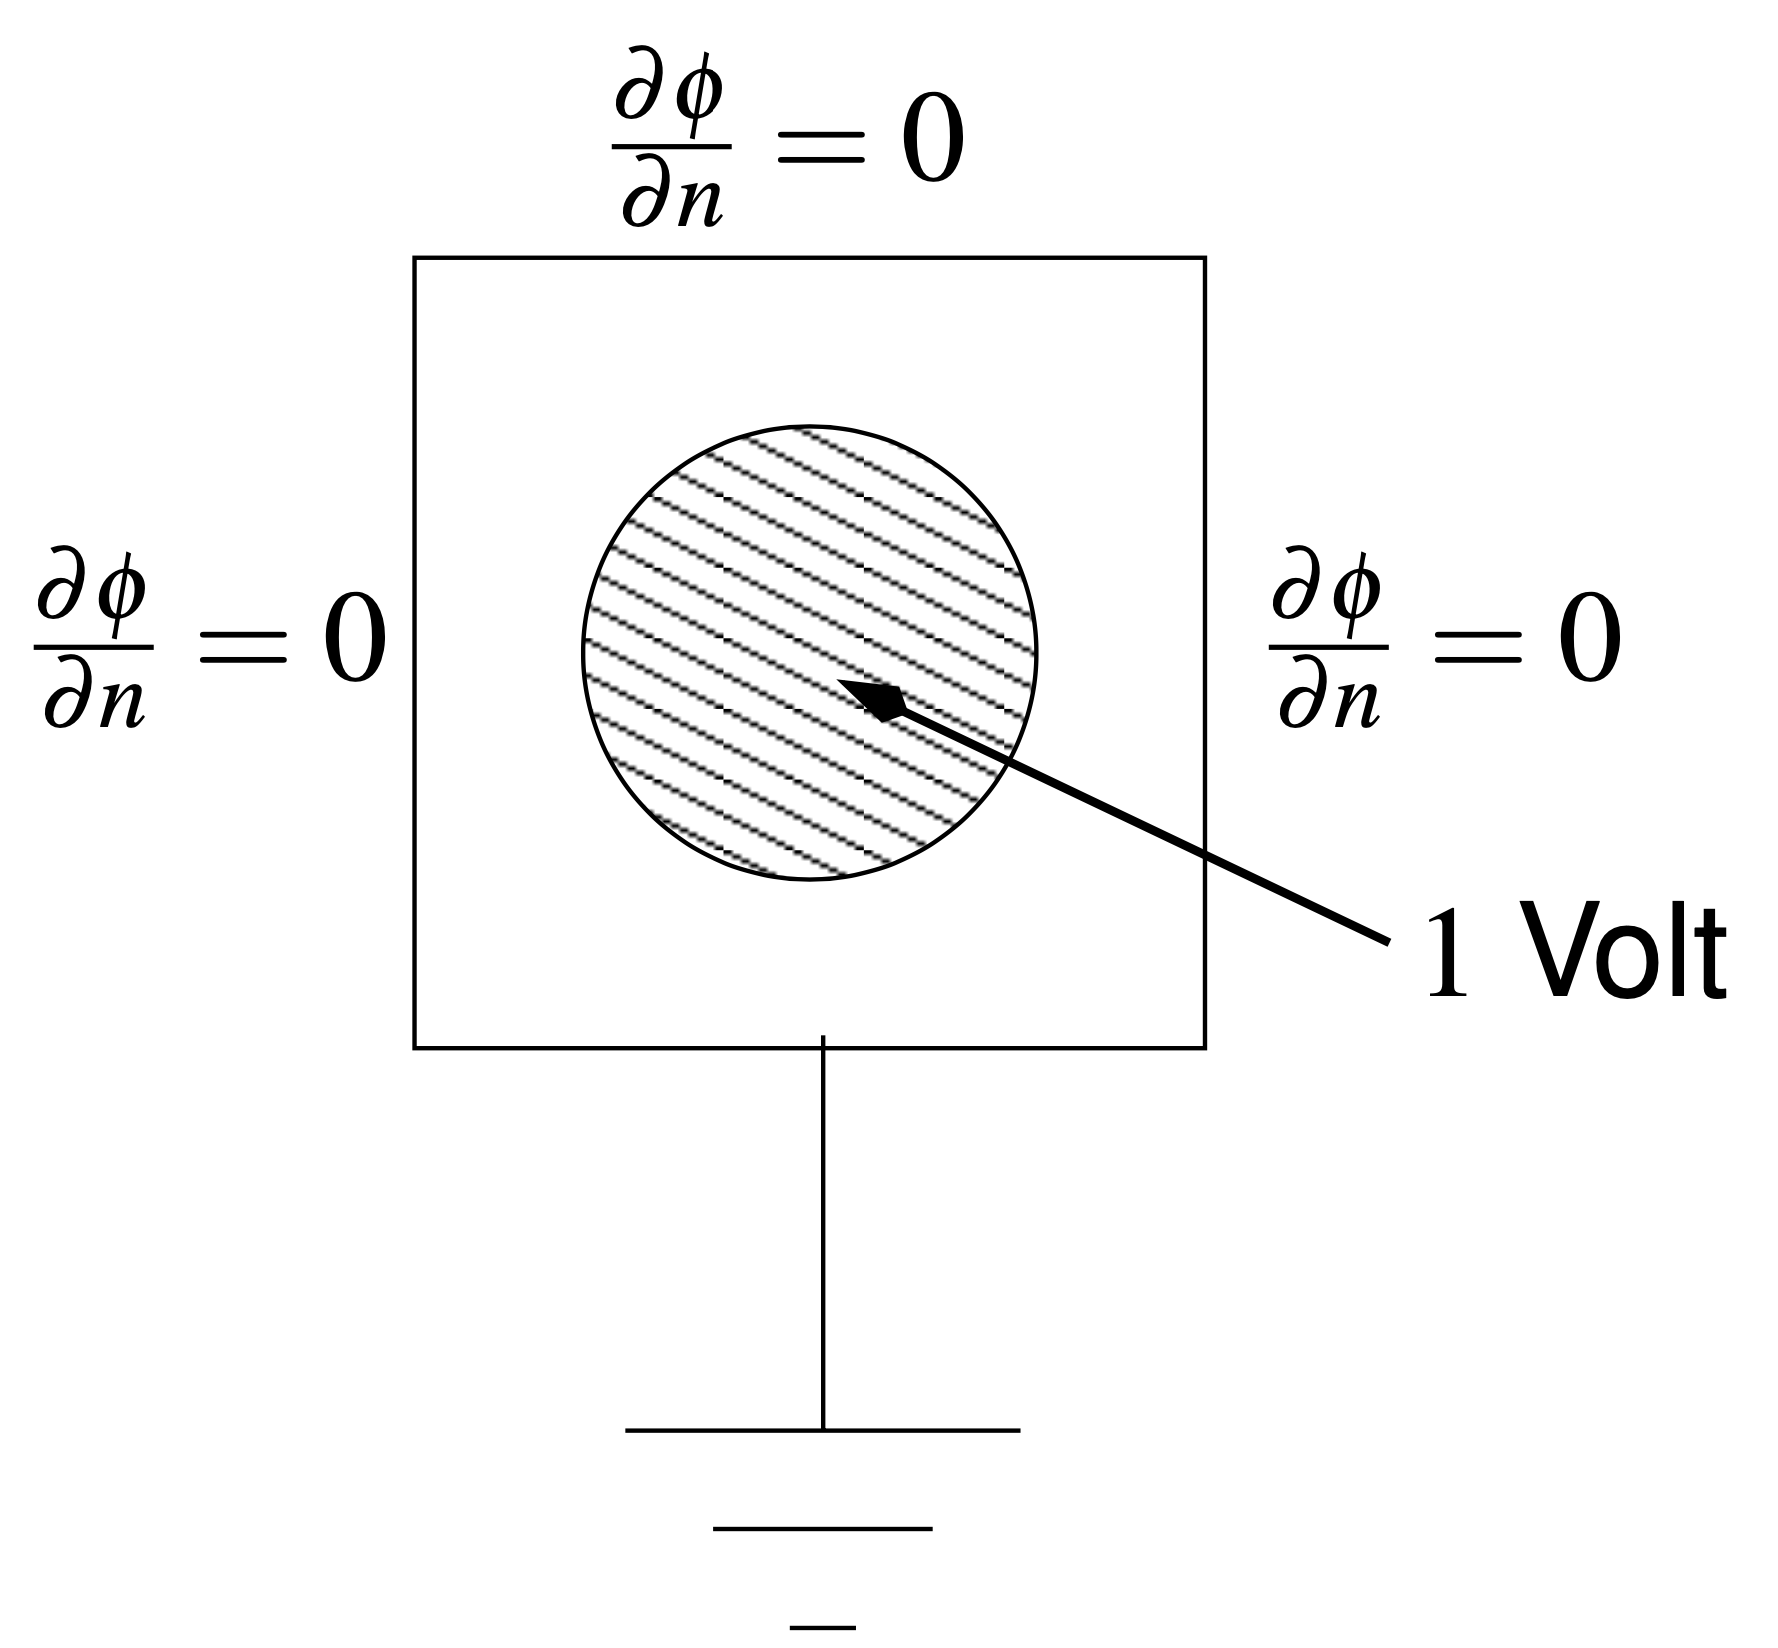
\includegraphics[scale=0.2]{plate.png}
\end{center}
\section{Calculating $\phi$ for the Conductor:}
Laplace’s equation is easily transformed into a difference equation.\par
The difference equation can be given as:
\begin{equation*}
\phi_{ij}=\frac{\phi_{i,j-1}+\phi_{i,j+1}+\phi_{i-1,j}+\phi_{i+1,j}}{4}
\end{equation*}and this can be easily implemented in python without using nested for loop as shown below. This is possible to perform by using vectorized for loops.\par
Initializing the array of phi:
\begin{equation}
\phi=\begin{bmatrix} 
      	0 & 0 & \cdots & 0 \\
        	0 & 0 & \cdots & 0 \\
            \vdots & \vdots & \ddots & \vdots \\
            0 & 0 & \cdots & 0 \\
        \end{bmatrix}
\end{equation}
\begin{verbatim}
Niter=1500    ### no. of iterations to be performed
phi = array([zeros(Ny)]*Nx)
for i in range(0,Niter):
	oldphi=phi.copy()
	phi[1:-1,1:-1]=0.25*(phi[1:-1,0:-2] phi[1:-1,2:]+phi[0:-2,1:-1]+phi[2:,1:-1])
	errors[i]=(abs(phi-oldphi)).max() ##calc. of errors with each iteration
\end{verbatim}
where, \par
$ii$ corresponds to the points in contact with the positive terminal of the supply in contact with the conductor and it is given using the $where()$ function as follows:

\begin{verbatim}
ii=where((X*X+Y*Y)<=(radius**2))
\end{verbatim}

\par
Specifying the resolution of the required potential on the conductor and the number of iterations to be performed is given through the input from the user. If it's not given, the defaults values we assume for calculating the potential is given as follows:
\begin{verbatim}
Nx=25; ## size along x
Ny=25; ## size along y
radius=8;  ## radius of central lead
Niter=1500; ## number of iterations to perform
\end{verbatim}
\par
And finally we have to assert the boundary conditions for each iteration :
\begin{verbatim}
	phi[ii]=1.0
	phi[-1]=0
	phi[1:-1,0]=phi[1:-1,1]
	phi[1:-1,-1]=phi[1:-1,-2]
	phi[0]=phi[1]
\end{verbatim}
\begingroup

\section{Computing the Errors in each Iteration:}

The coefficients are stored in the fashion,\par 
\begin{equation*}
errors=\begin{bmatrix} 
e_0 & e_1 & e_2 & e_3 &\cdots & e_{1498} &  e_{1499}
 \end{bmatrix}
 \end{equation*}
 Where, $e_i$ is the error while iterating the loop for $i^{th}$ time.\par
 And this calculated as follows:
 \begin{verbatim}
 errors=zeros(Niter)
 errors[i]=(abs(phi-oldphi)).max()   ##is executed in the for loop
 \end{verbatim}
 \par
 
\section{Computing the Current Density:}

The Current Density $\vec{j}$, is defined as follows:
\begin{equation*}
\vec{j_x} = \sigma . (-\frac{\partial \phi}{\partial x})
\end{equation*}

As we are to plot the current density vectors, so we drop the $\sigma$ term as it contributes to the magnitude of vectors only.

And this is numerically translated as follows:
\begin{align*}
j_{x,ij}=\frac{1}{2} (\phi_{i,j-1}-\phi_{i,j+1}) \\
j_{y,ij}=\frac{1}{2} (\phi_{i-1,j}-\phi_{i+1,j})\\
\end{align*}


And this is implemented in python as follows:
\begin{verbatim}
j_x = array([zeros(Ny)]*Nx)
j_y = array([zeros(Ny)]*Nx)

j_x[:,1:-1]=0.5*(phi[:,0:-2]-phi[:,2:])
j_y[1:-1,:]=0.5*(-phi[0:-2,:]+phi[2:,:])		#calculating currrent density
j_y[-1]=(-phi[-2])
\end{verbatim}
% \vspace{1cm}
\newpage 

\section{Least Squares Approach to fit the Errors to the Exponential Form:}
So, as the errors are stored in the array named - $errors$

 We want to fit the errors to the form:
 \begin{equation*}
 e=Ae^{Bx}
 \end{equation*}
 Where, x is the number of iterations, and e is the error. Thus, we need to calculate the A and B constants for the acquired errors.\par
 The above equation can be modified to the form:
 \begin{equation*}
 log(e) = log(A) +Bx
 \end{equation*}
 Thus, we need tho fing the values of log(A) and B by giving the $log(errors)$ to the $lstsq$ funciton.\par
 As the coefficient of $log(A)$ is $1$, and the coefficient of $B$ is $e$, so we create the $2D$ arrays as follows:
 \begin{verbatim}
 samples=array([zeros(2)]*Niter)
samples[:,0]=1
iter=arange(1,Niter+1,1)
samples[:,1]=iter
 \end{verbatim}
 
 
 \subsection{Fitting the Entire Vector of Errors:}

\begin{verbatim}
err_coeff=lstsq( samples , log(errors) ,rcond=-1)[0]
A=exp(err_coeff[0])
B=err_coeff[1]
\end{verbatim}


 \subsection{Fitting the Errors for the number of iterations exceeding $500$:}

\begin{verbatim}
err_coeff_500=lstsq( samples[500:] , log(errors[500:]) ,rcond=-1)[0]
A_500=exp(err_coeff[0])
B_500=err_coeff_500[1]
\end{verbatim}

    
\subsection{Least Squares Method}
The method of least squares is a standard approach in regression analysis to approximate the solution of overdetermined systems (sets of equations in which there are more equations than unknowns) by minimizing the sum of the squares of the residuals made in the results of every single equation.
The most important application is in data fitting. The best fit in the least-squares sense minimizes the sum of squared residuals (a residual being: the difference between an observed value, and the fitted value provided by a model).\par
So, as the coefficients are varied to minimize the error, we differentiate the error wrt. each coefficient and equate it to zero, in order to obtain the vector of optimal coefficients ($p_i 's$).\par
And in python, in scipy.linalg library, there is a dedicated function, named $lstsq()$ [leastsqares], which accepts the arguments as : $lstsq(F,x)$

\newpage
\section{Plots of Functions and Coefficients:}
\begin{verbatim}
n=arange(0,Niter,50)
\end{verbatim}
\subsection{Semilog plot of Errors for all iterations along with the Estimated Functions:}
\begin{verbatim}
title('Semilog plot of errors with no. of Iterations')
semilogy(n,errors[::50],color='blue',label= 'Errors')
semilogy(n,e(n,A,B),color='green',label= 'Fit of Errors') 
xlabel(r'$N_{iter}$' ' ' '$\longrightarrow$',size=15)
semilogy(n,e(n,A_500,B_500),color='orange',label= 'Fit of Errors after 500')
legend(loc="upper right")
\end{verbatim}
{\centering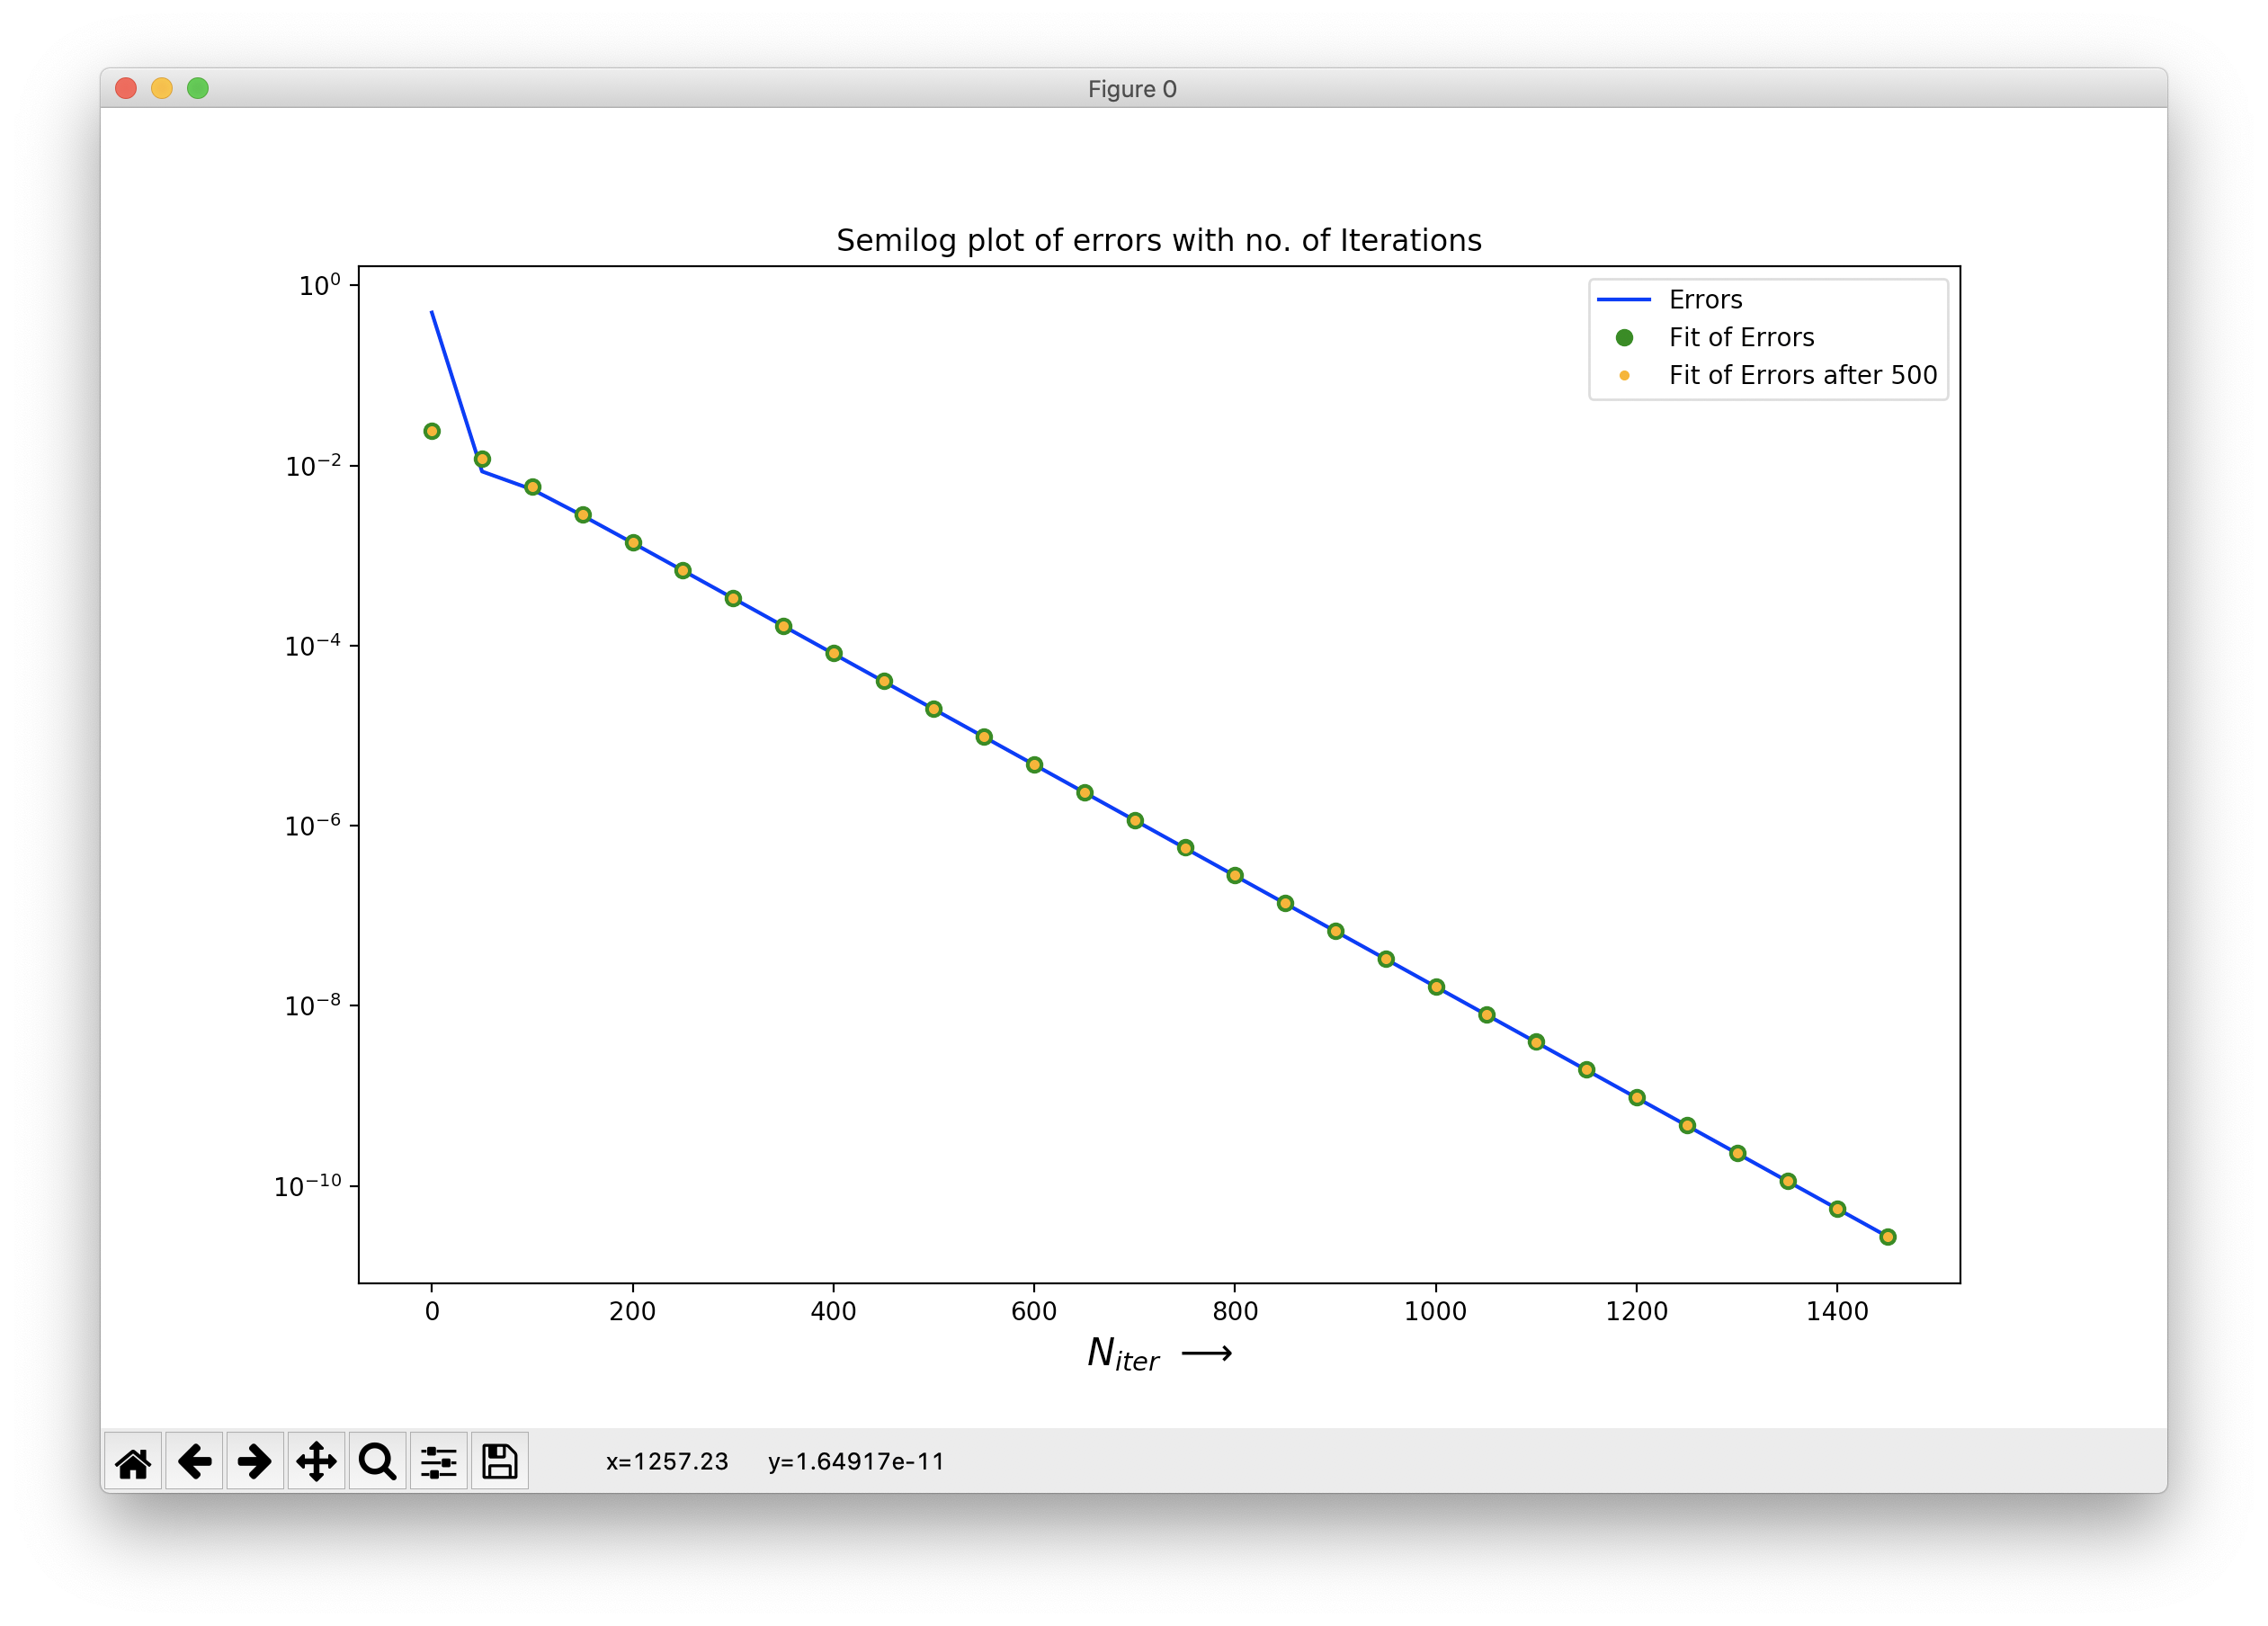
\includegraphics[scale=0.4]{Figure_0.png}}
\newpage

\subsection{Loglog plot of Errors for all iterations along with the Estimated Functions:}
\begin{verbatim}
title('Loglog plot of errors with no. of iterations')
loglog(n,errors[n],color='blue',label= 'Errors')
loglog(n,e(n,A,B),color='green',label= 'Fit of Errors') 
xlabel(r'$N_{iter}$' ' ' '$\longrightarrow$',size=15)
loglog(n,e(n,A_500,B_500),color='orange',label= 'Fit of Errors after 500')
legend(loc="upper right")
\end{verbatim}
{\centering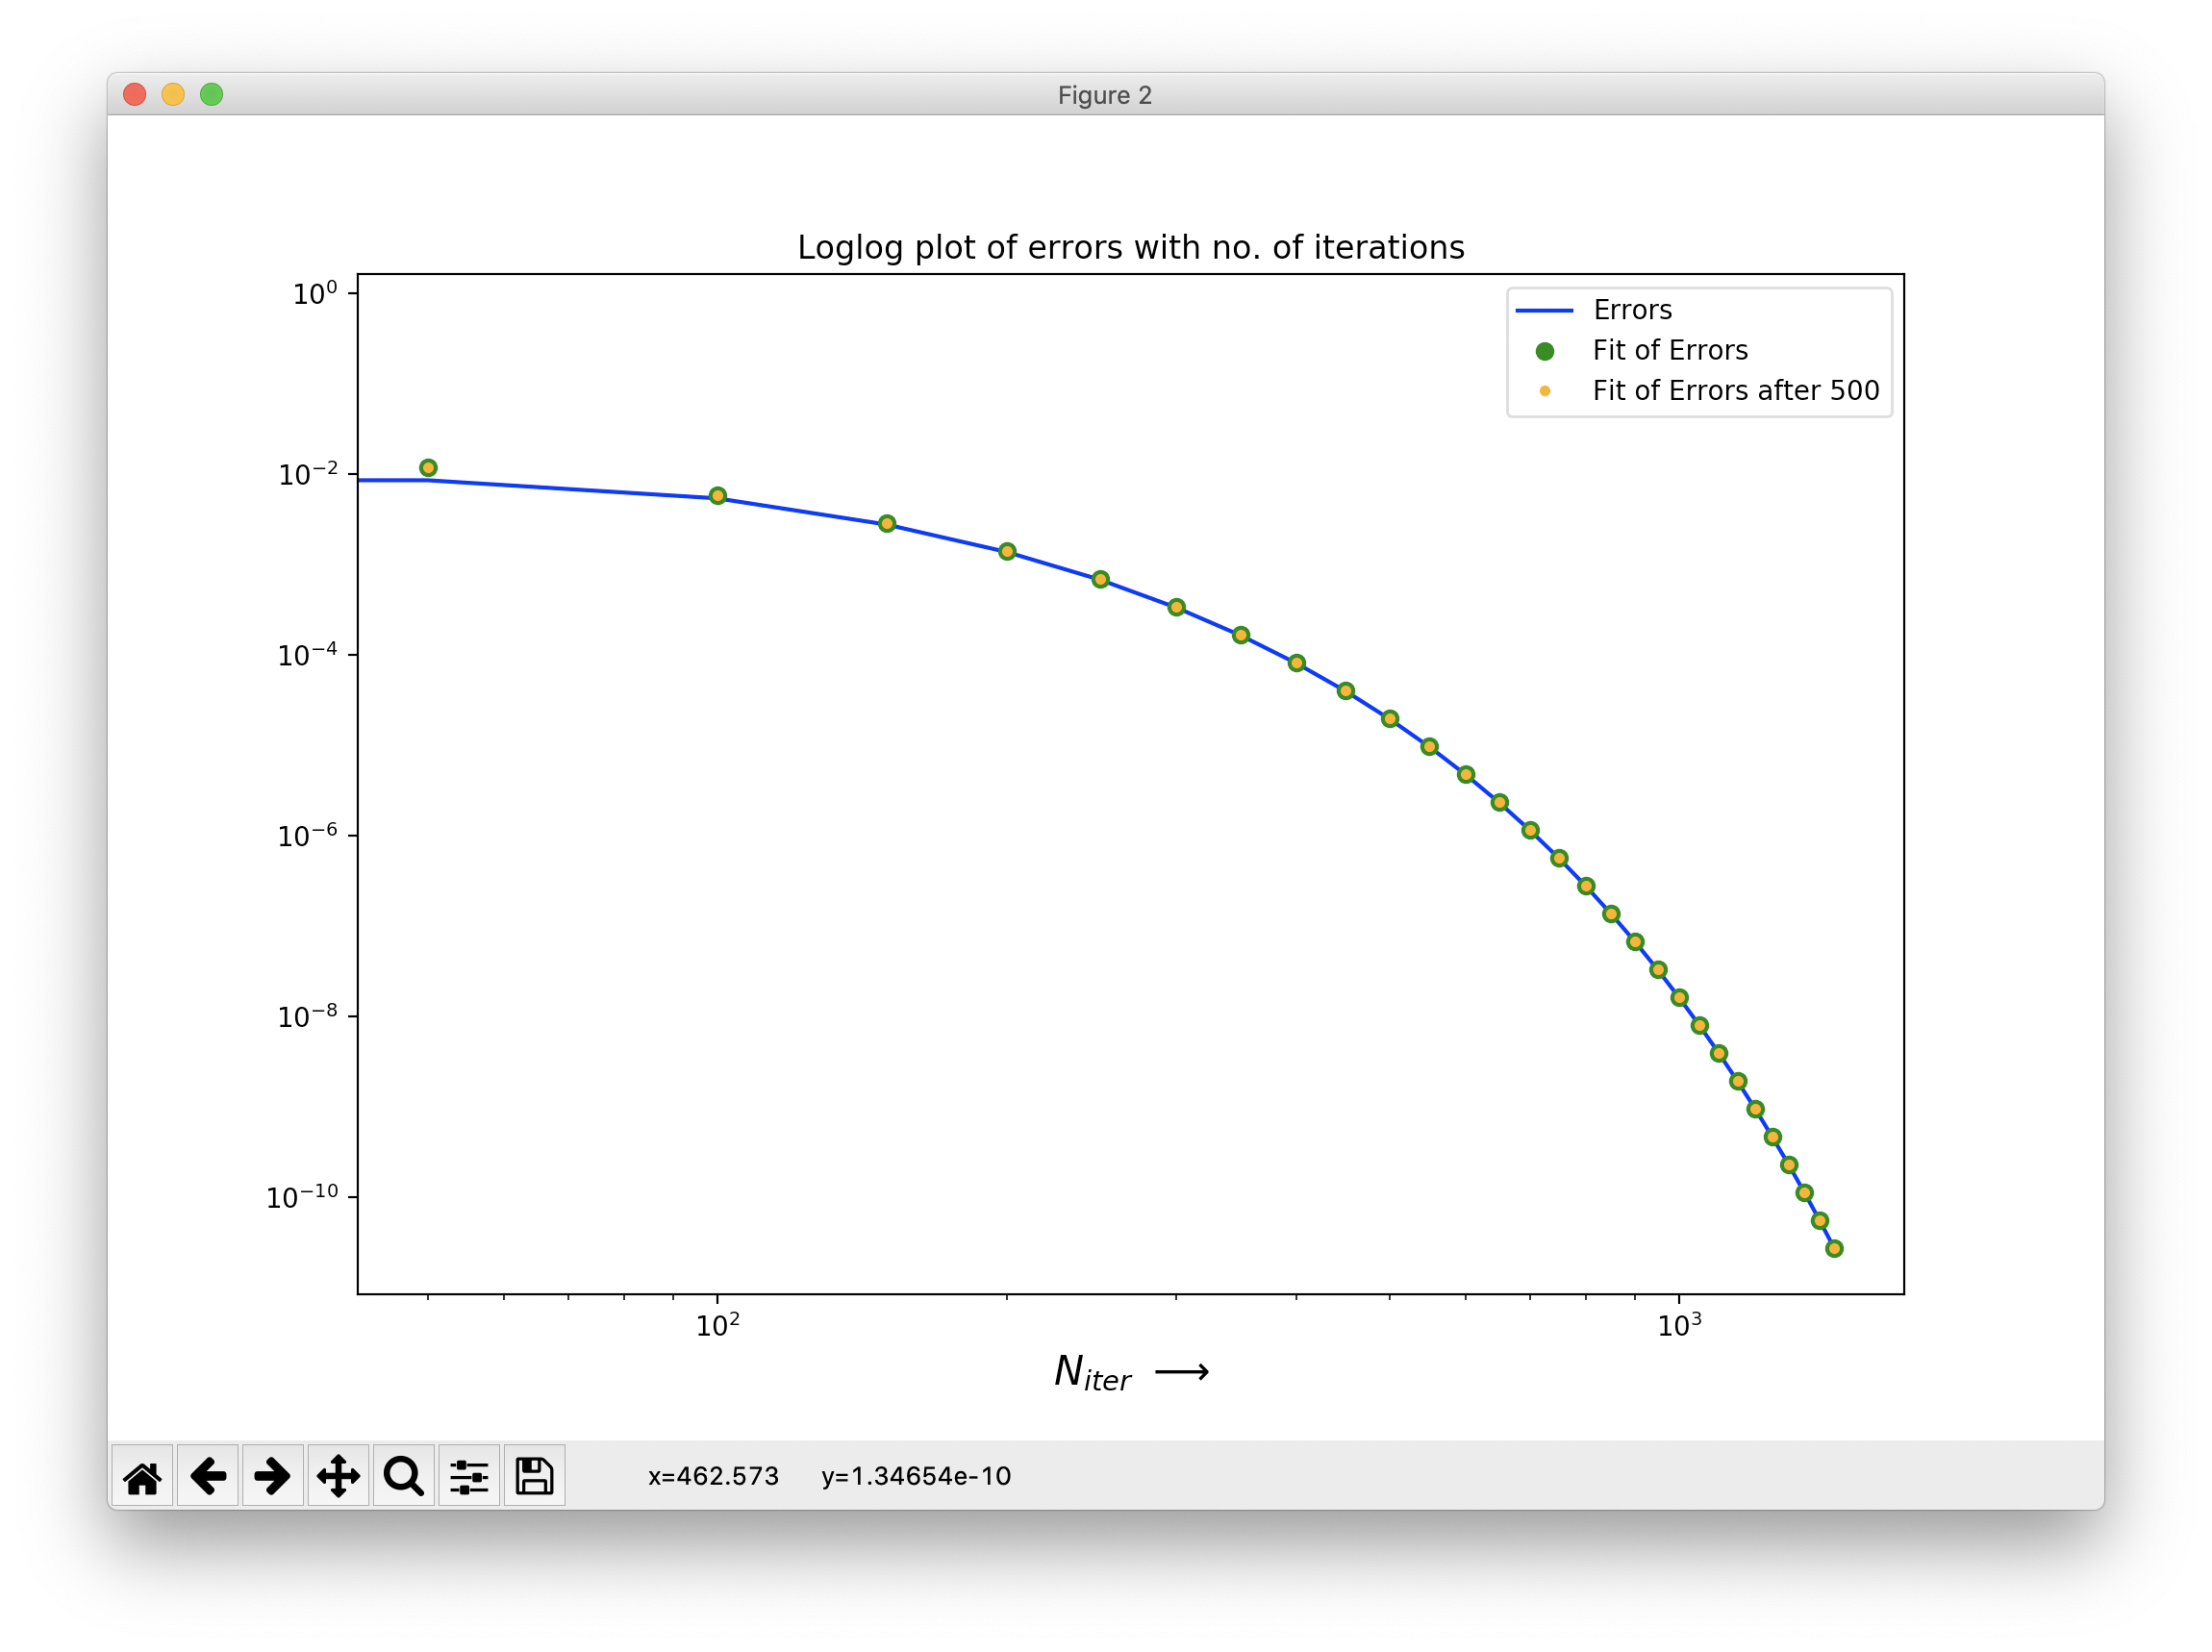
\includegraphics[scale=0.4]{Figure_2.png}}
\newpage
\subsection{The 3-D surface plot of the Potential - $\phi$:}
\begin{verbatim}
fig4=figure(4) # open a new figure
ax=p3.Axes3D(fig4) # Axes3D is the means to do a surface plot
title('The 3-D surface plot of the potential')
surf = ax.plot_surface(-Y, -X, phi, rstride=1, cstride=1, cmap=cm.jet)
\end{verbatim}
{\centering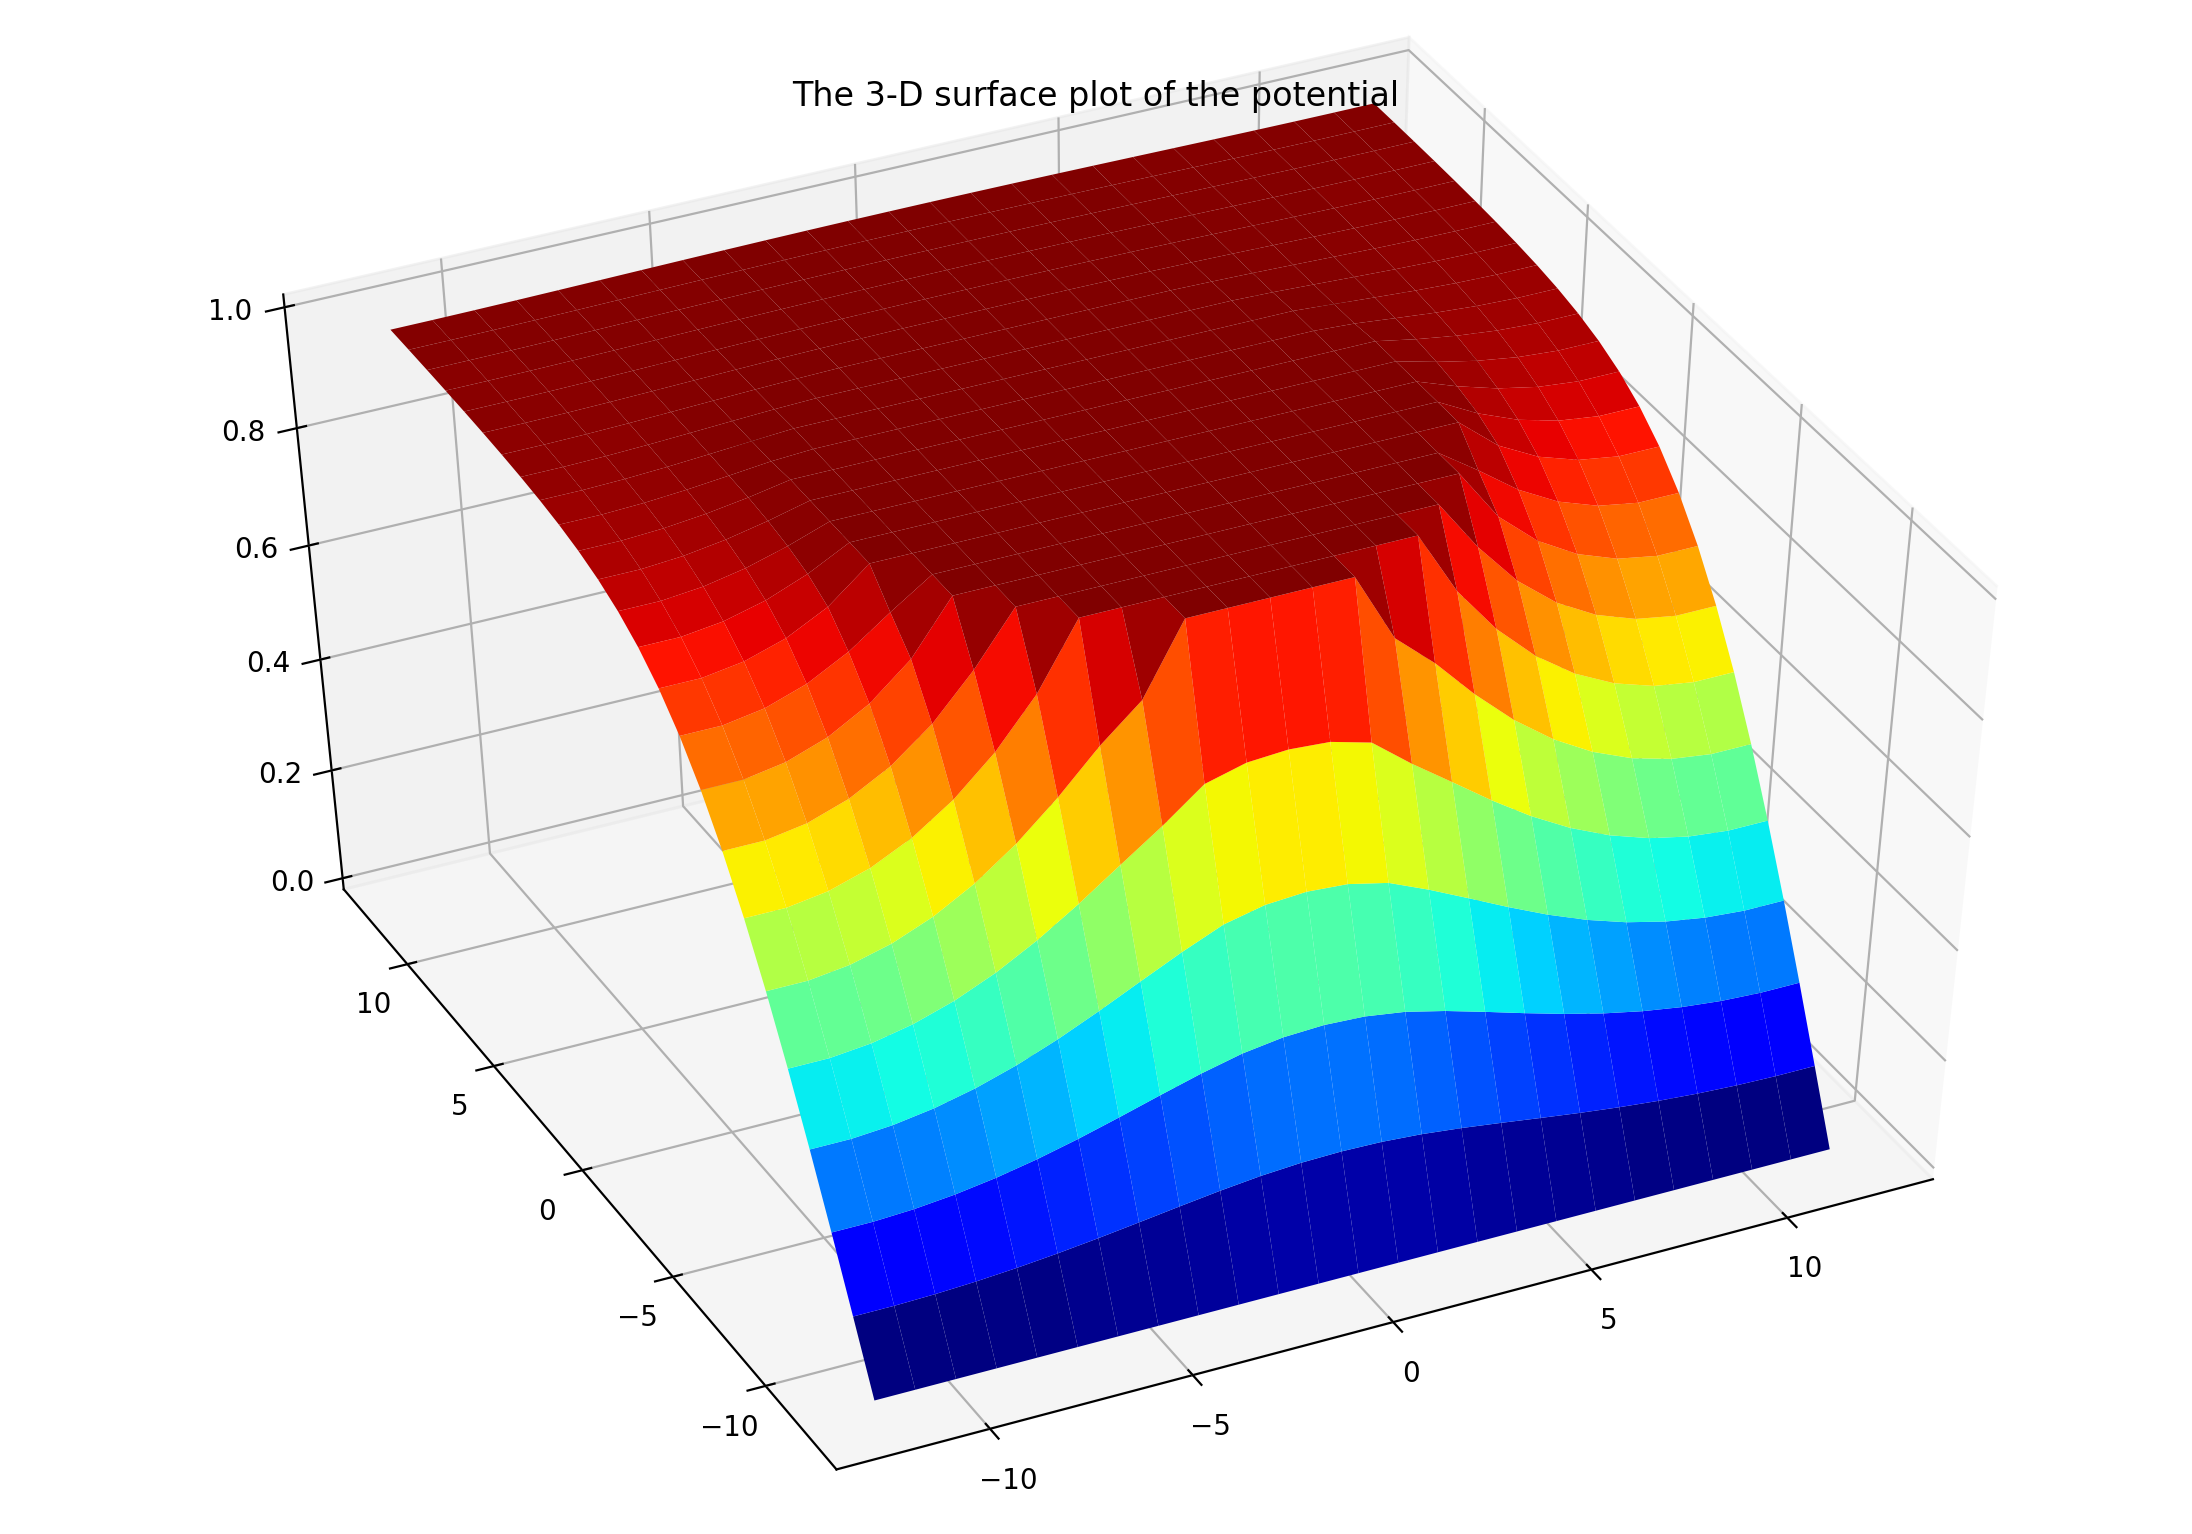
\includegraphics[scale=0.7]{Figure_4.png}}
\newpage
\subsection{Contour plot of $\phi_{ij}$ :}
\begin{verbatim}
cp = plt.contour(Y, -X, phi, linestyles='-')
clabel(cp, inline=True,fontsize=10)
xlabel('Ground',size=15)
title(r'Contour plot of $V_{ij}$ ' )
\end{verbatim}

{\centering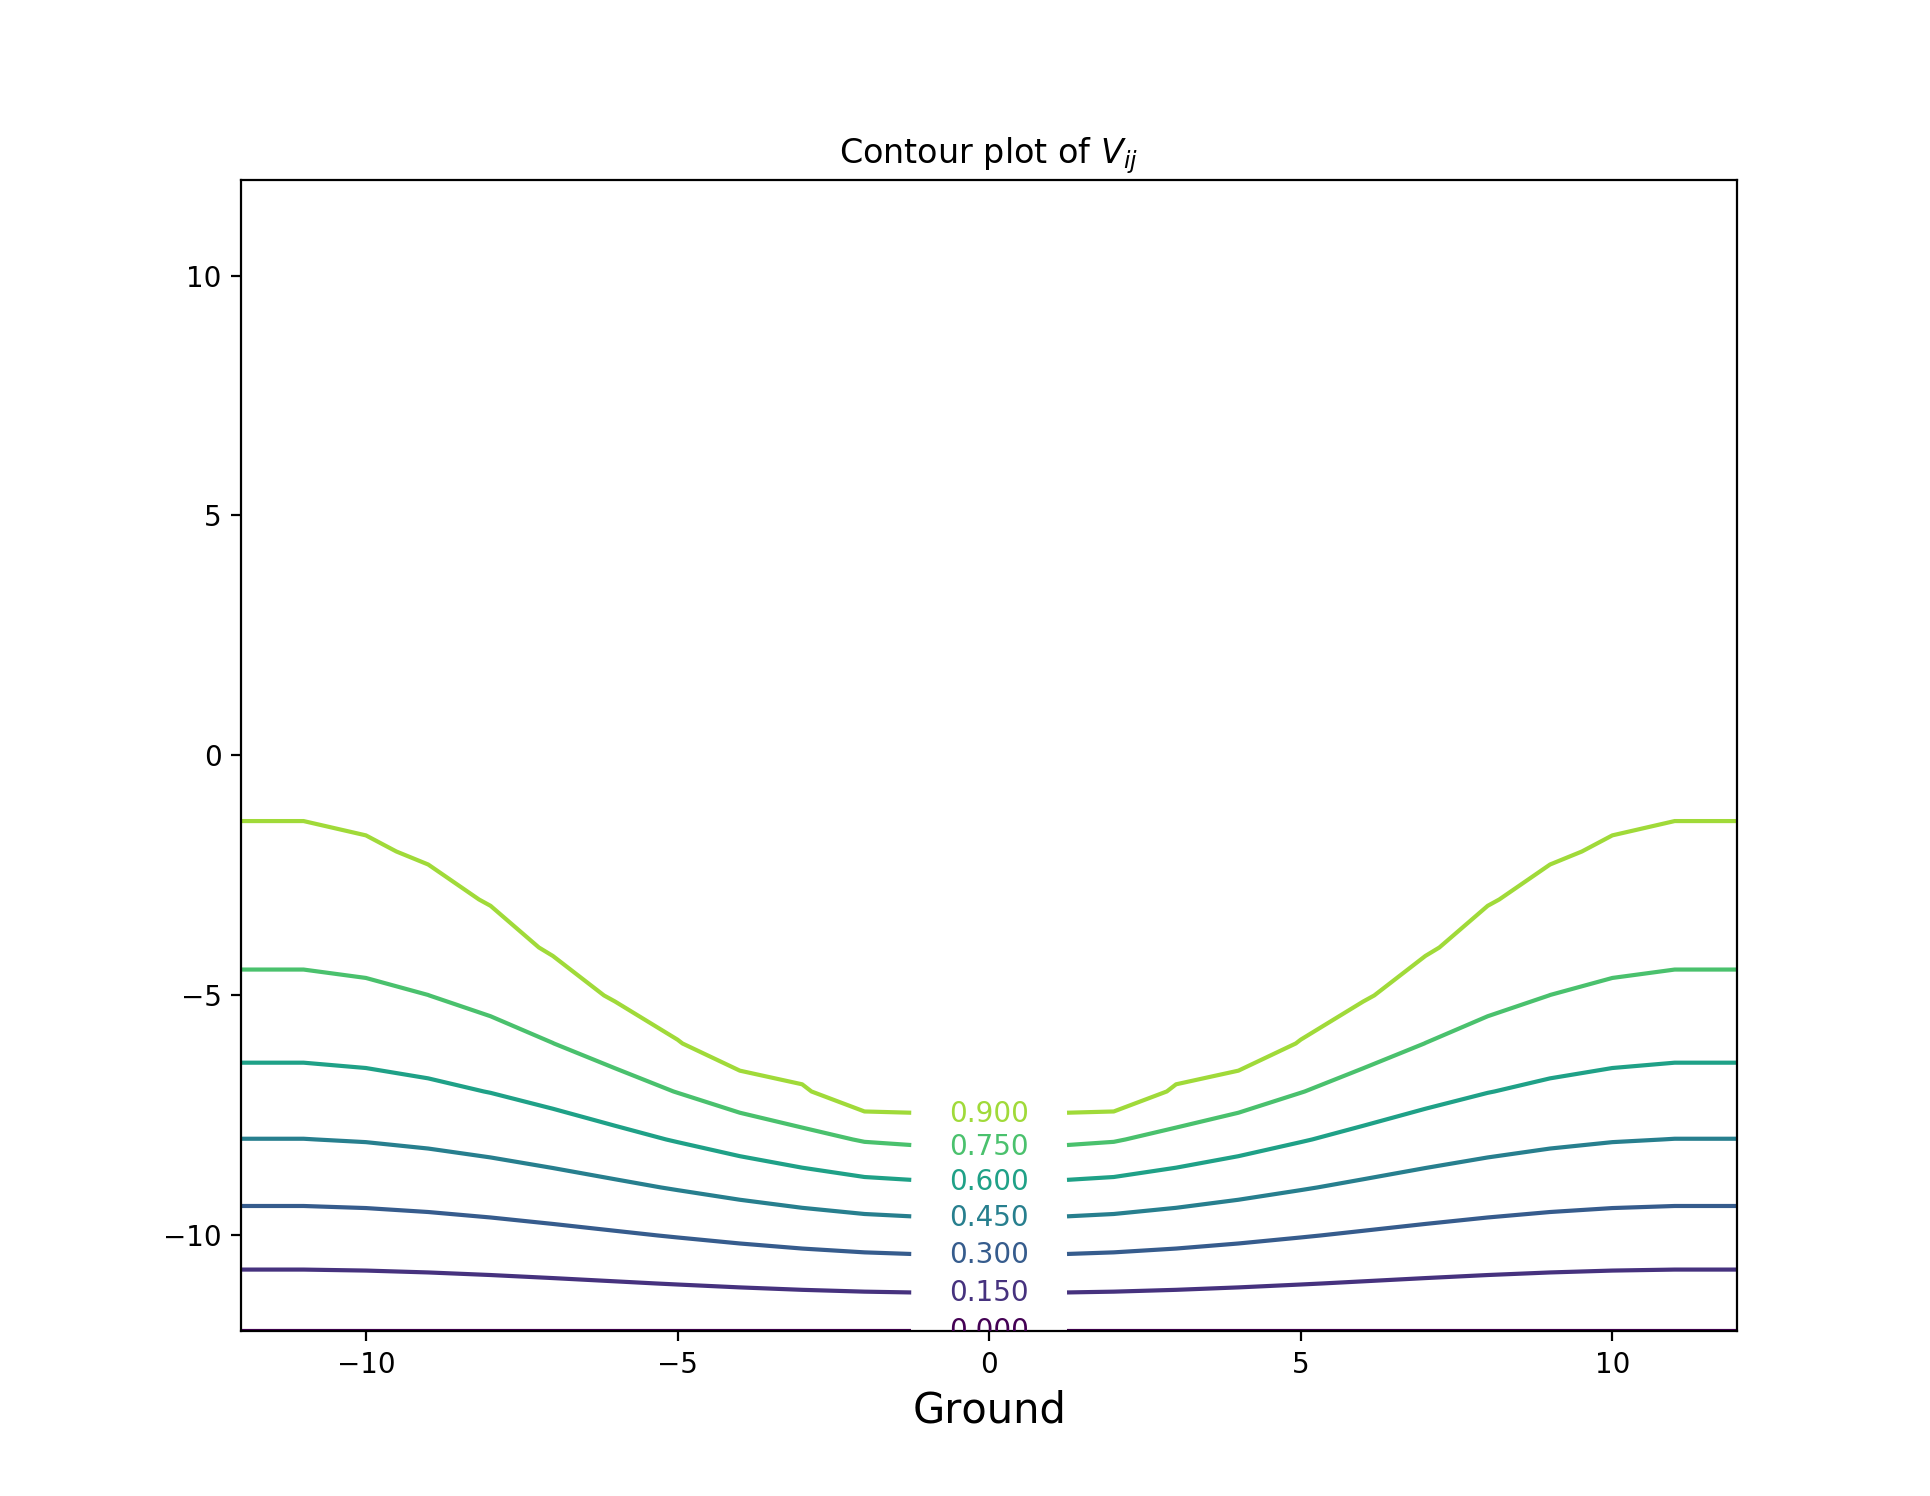
\includegraphics[scale=0.7]{Figure_5.png}}
\newpage
\subsection{Vector plot of Current Density:}
\begin{verbatim}
title('Vector plot of Current Density')
q=quiver(-y,-x,j_x,j_y, scale=1.2, scale_units='inches',label="J - Vectors")
scatter(X[ii],Y[ii],color='red',label="1 Volt Region")
legend(loc="upper right")
show()
\end{verbatim}
As, we also need to plot the $1V$ potential region, we use the scatter command to do that.\\
{\centering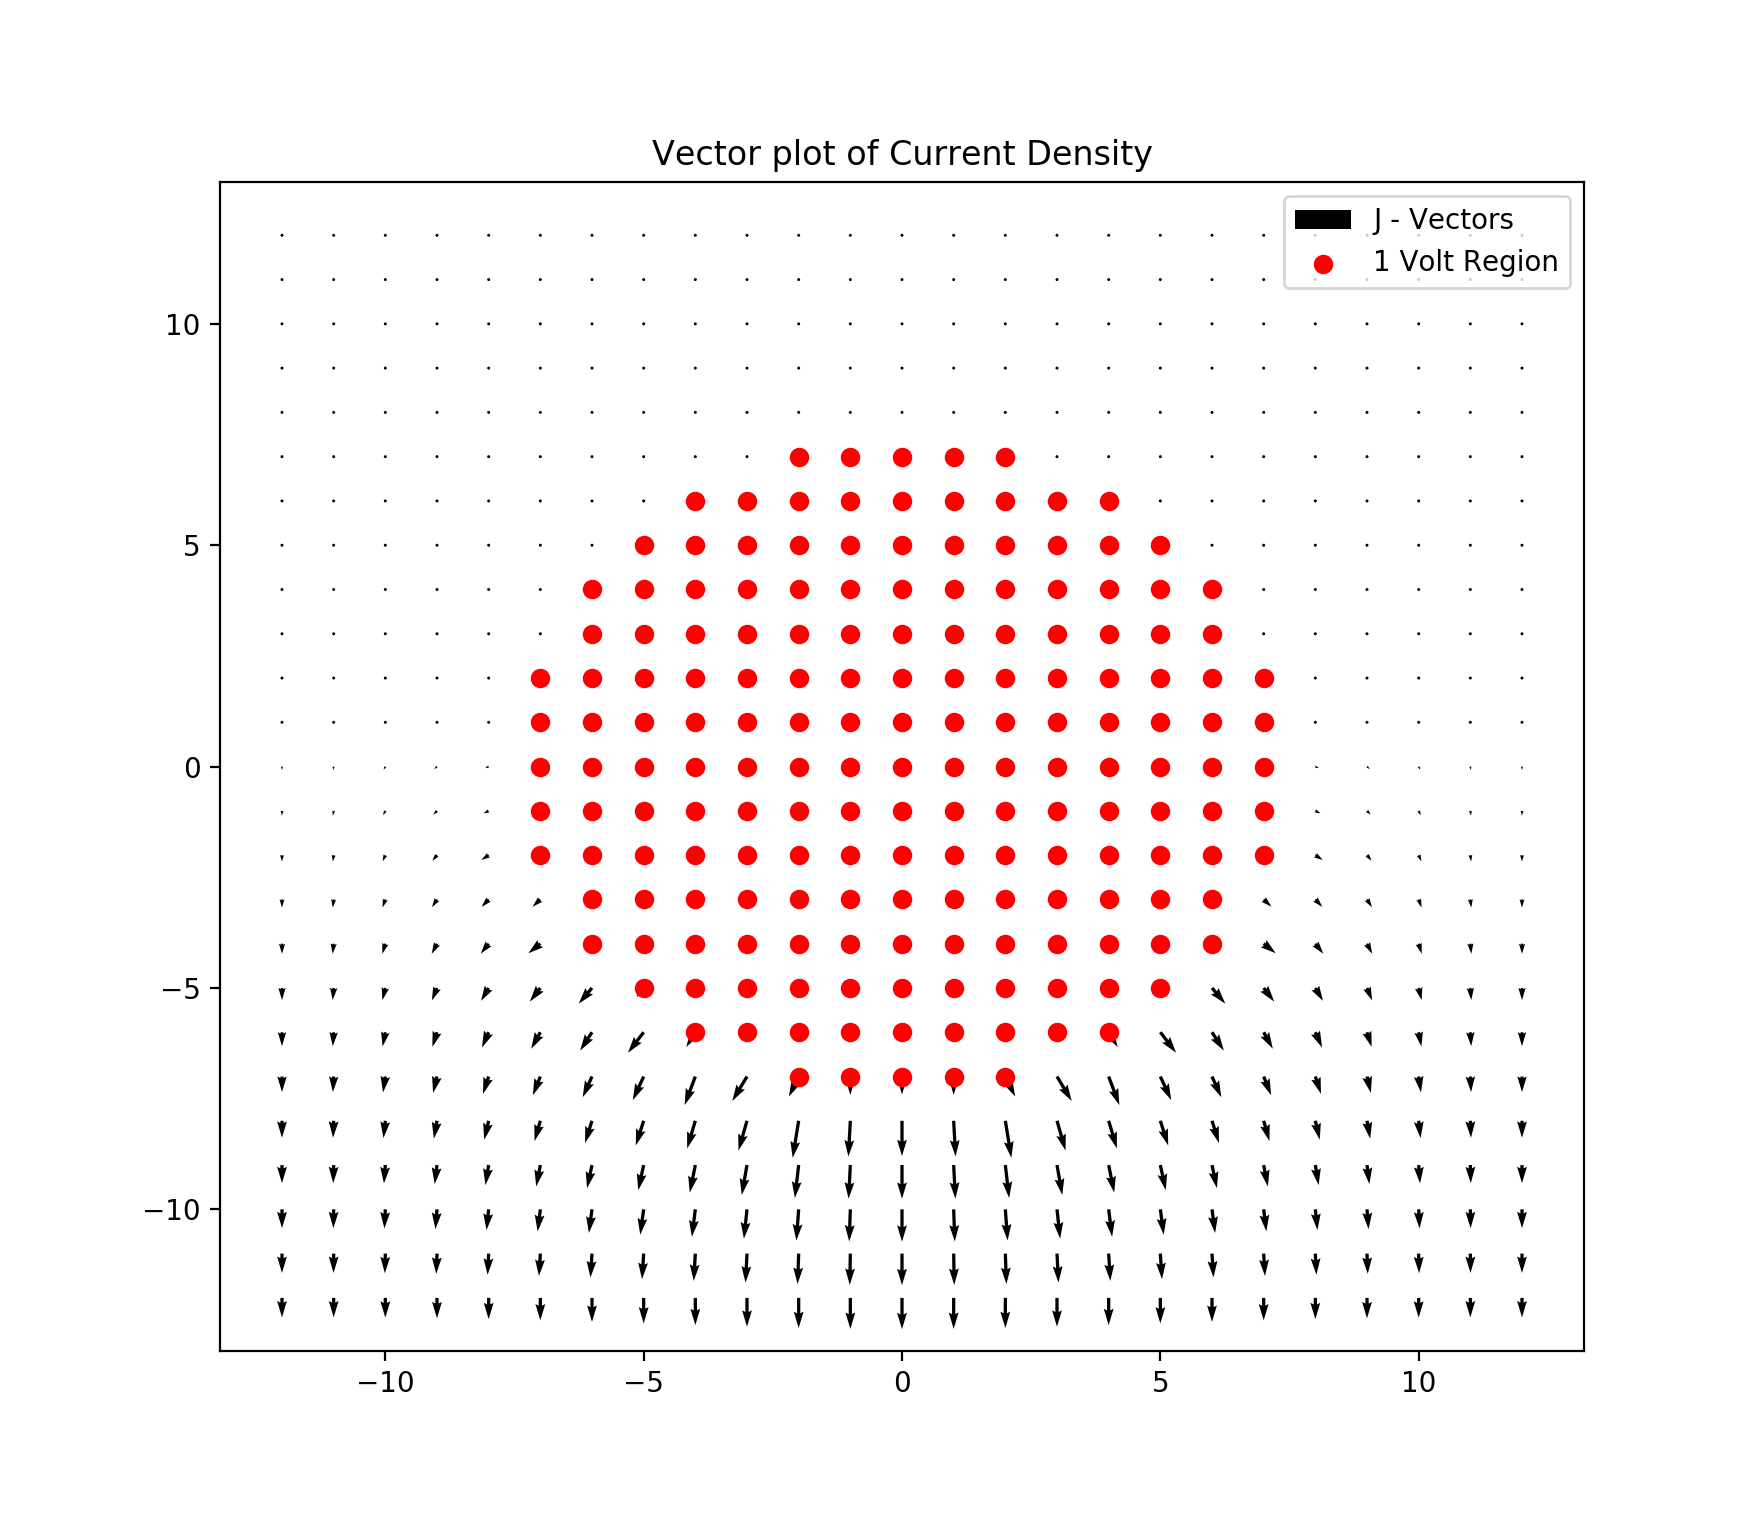
\includegraphics[scale=0.7]{Figure_6.png}}

\chapter{Conclusions}
\section{On Current Density:}
As the entire current flows through the ground, thus the lower part has a more density of the current, where as the top plate is like a \textit{floating node}-as it is not connected to any other reference potential node, so the current doesn't flow out of the top edge.\\
Thus the current which will go in the upper half of the plate, must return downwards, as no charge gets accumulated in the case of steady state assumption.\\
Hence the |$\vec{j}$| is more denser in the bottom plate and less denser in the upper plate.

% \pagebreak

\end{document}



